% paper/sections/14_benchmarks.tex
%
% §14  二相流ベンチマーク — physical benchmark set
%

\section{二相流ベンチマーク}
\label{sec:validation}
\label{sec:benchmarks}

第~\ref{sec:verification}章では，単相 NS，静止液滴，密度比 sweep，
非一様格子，CLS 強変形移流を用いて，個々の離散閉包が
設計通りに働く範囲を確認した．
本章では，その部品検証を越えて，移動界面・表面張力・変密度投影・浮力が
同時に作用する物理ベンチマークを扱う．
対象は，毛管波，Rayleigh--Lamb 型振動液滴，単一気泡上昇，
および Rayleigh--Taylor 不安定性の 4 本である．

本章のナラティブは，界面力学の難しさを段階的に増やすことで統一する．
毛管波では，平坦界面の小振幅復元力が pressure-jump の符号と面勾配に正しく入るかを見る．
振動液滴では，閉じた界面が往復運動することで，表面エネルギー，運動エネルギー，
移流項，粘性項の交換を読む．
単一気泡上昇では，表面張力に加えて浮力残差と pressure projection の共有 face locus を読むが，
本稿では形状破綻が現れる前の初期窓 $0\le t\le0.03\,\mathrm{s}$ に掲載範囲を限定する．
Rayleigh--Taylor では，浮力が安定化ではなく不安定成長を作る配置で，
線形増幅から非線形形状形成までを追う．
静止円形液滴は production-stack static gate を含めて第~\ref{sec:verification}章で扱ったため，
本章では重複させない．

% ═══════════════════════════════════════════════════════════════════
\subsection{共通数値スタックと判定方針}
\label{sec:val_grid_policy}
% ═══════════════════════════════════════════════════════════════════

4 本のベンチマークは，実験ごとに幾何・境界条件・重力を変える一方で，
次の共通数値構成を共有する：
\begin{itemize}[noitemsep,leftmargin=2em]
  \item interface-fitted 非一様格子 $\alpha=2$，
        移動界面追従ケースでは毎 step rebuild，
  \item FCCD 保存形界面輸送 + TVD--RK3，
  \item UCCD6 対流 + IMEX--BDF2，CCD 粘性 + implicit--BDF2 + defect correction，
  \item アクティブ幾何毛管分解：
        幾何セル分率 $q_C$ を主状態とし，
        bundle Young--Laplace work と
        pressure-component Hodge reaction で毛管面共鎖を構成，
  \item Ridge--Eikonal 再初期化を各ベンチマークの設定に従って適用し，
        本章の毛管波と振動液滴では毎 step profile restoration を行う，
  \item 向き付き pressure-jump
        $j_{gl}=p_g-p_l=-\sigma\kappa_{lg}$ を現在の切断面 face law で評価する
        phase-separated FCCD PPE + affine jump，
  \item 射影と同じ面フラックスと正準面速度による界面輸送，
        および格子再構築時の投影済み面共鎖移送．
\end{itemize}
したがって本章で比較するのは solver option の違いではなく，
同じ離散閉包を異なる物理状況へ置いたときの応答である．

非一様格子を採用できる条件は，格子密度比 $\alpha$ そのものではなく，
投影・浮力残差・速度補正・界面輸送が同じ面位置を共有することである．
投影形 PPE が $D_fA_fG_f$ を用い，solve 形では $-D_fA_fG_f$ を解くなら，
corrector は同じ $A_fG_f$ で速度を補正し，
浮力残差も同じ face-gradient chain 上で評価する
（式~\eqref{eq:same_face_projection_closure}）．
さらに，projection で得た正準面速度を
式~\eqref{eq:projection_native_psi_transport} に直接渡す．
節点へ再構成した速度から界面フラックスを作り直す経路は，
同じ離散化の別表現ではなく，面速度空間の契約の破れである．

各ベンチマークは，時間履歴診断と snapshot 診断を組み合わせて判定する．
時間履歴では体積保存，運動エネルギー，界面振幅，変形量，重心，
平均上昇速度などを読む．
snapshot では $\psi$，速度場，圧力代表を同じ時刻で読み，
体積保存だけでは見えない pressure-jump/buoyancy の不整合を検出する．
判定は，単なる完走ではなく，
\textbf{保存性，理論で決まる初期応答，長時間の有界性，形状発展の物理的一貫性}
の 4 軸で行う．

% ═══════════════════════════════════════════════════════════════════
\subsection{毛管波：平坦界面の毛管復元力}
\label{sec:val_capillary}
% ═══════════════════════════════════════════════════════════════════

\subsubsection{設定と理論基準}

毛管波ベンチマークは，平坦界面に小振幅の正弦波摂動を与え，
表面張力による復元振動を観察する最も単純な移動界面テストである．
初期界面は
\begin{equation}
  y_\Gamma(x,0)=y_0 + A_0\cos(kx+\theta_0),
  \qquad
  k=\frac{2\pi m}{L_x}.
  \label{eq:capillary_wave_initial}
\end{equation}
初期条件は水--空気の実スケールとして
$y_0=0.01\,\mathrm{m}$，$A_0=2.0\times10^{-4}\,\mathrm{m}$，
$m=2$，$L_x=0.02\,\mathrm{m}$，$\theta_0=0$ とする．
したがって波長は $\lambda=L_x/m=0.01\,\mathrm{m}$ である．
上下壁の間に置かれた有限深さ二流体の小振幅理論では
\begin{equation}
  \omega^2
  = \frac{\sigma k^3}
         {\rho_l\coth(kh_l)+\rho_g\coth(kh_g)},
  \qquad
  h_l=h_g=0.01\,\mathrm{m},\quad g=0,
  \label{eq:flat_capillary_dispersion}
\end{equation}
を第一基準に置く~\cite{Prosperetti1981}．
この設定では $k=628.318530718\,\mathrm{m^{-1}}$ であり，
\[
  \omega_\sigma
  =134.419859151\,\mathrm{s^{-1}},\qquad
  T_\sigma=\frac{2\pi}{\omega_\sigma}=0.046742983863\,\mathrm{s}
\]
を連続体の基準時刻とする．
ただし，論文に掲載する 2 次元 snapshot は，
非負 envelope ではなく，計算された符号付き mode-2 界面振幅
\texttt{signed\_interface\_amplitude} の戻り窓を使って選ぶ．
すなわち起点，上側から平坦化する点，下側最大，ふたたび平坦化する点，
上側へ戻る終点の 5 点を
\[
  t=0.000018444039,\ 0.008913124850,\ 0.017699729500,\ 0.026639206900,\
  0.035379718894\ \mathrm{s}
\]
に対応させる．
本ケースでは重力を切るため，初期加速度は曲率と圧力ジャンプだけで決まる．
向き付き規約
\[
  \psi=1\ \text{液相},\quad \psi=0\ \text{気相},\quad
  \kappa_{lg}=\nabla_\Gamma\!\cdot\hat{\bm n}_{lg},\quad
  j_{gl}=p_g-p_l=-\sigma\kappa_{lg}
\]
に従えば，山の初期加速度は復元向きでなければならない．

\begin{itemize}[noitemsep,leftmargin=2em]
  \item グリッド：$[0,0.02]^2\,\mathrm{m}^2$，$32^2$，$x$ 周期，$y$ 壁面，
        interface/wall fitted 非一様格子
  \item 物性：$\rho_l=998.2\,\mathrm{kg/m^3}$，
        $\rho_g=1.204\,\mathrm{kg/m^3}$，
        $\mu_l=1.002\times10^{-3}\,\mathrm{Pa\,s}$，
        $\mu_g=1.825\times10^{-5}\,\mathrm{Pa\,s}$，
        $\sigma=0.0728\,\mathrm{N/m}$，$g=0$
  \item 時間：掲載窓 $T=0.035379718894\,\mathrm{s}$，
        理論 CFL multiplier $1.0$
  \item 出力：\texttt{signed\_interface\_amplitude}，
        \texttt{volume\_conservation}，\texttt{kinetic\_energy}，
        上側最大，ゼロ交差，下側最大，ゼロ交差，上側最大近傍の
        $\psi$/速度/圧力 snapshot
\end{itemize}

\subsubsection{結果と判定}

N=32 の掲載窓 run は $1623$ samples で
$t=0.035379718894\,\mathrm{s}$ に到達し，
すべての保存診断と snapshot field は有限値を保った．
CFL は全区間で毛管制限が支配し，
$dt$ は $1.844\times10^{-5}$--$2.326\times10^{-5}\,\mathrm{s}$ の範囲に留まった．
\texttt{signed\_interface\_amplitude} は初期離散値
$2.0058\times10^{-4}\,\mathrm{m}$ から最小
$-1.9730\times10^{-4}\,\mathrm{m}$ へ進み，
終端で $1.9199\times10^{-4}\,\mathrm{m}$ へ戻る
（最大 $2.0076\times10^{-4}\,\mathrm{m}$）．
この符号付き診断を用いることで，非負 envelope の
\texttt{interface\_amplitude} が符号を折り返して見かけ上短い周期を作る問題を避ける．
運動エネルギーは
$3.402\times10^{-11}$ から最大 $1.659\times10^{-5}$ まで増加し，
終端では $8.964\times10^{-6}$ である．
体積ドリフトは最大 $1.556\times10^{-8}$，
終端 $1.132\times10^{-9}$ であり，掲載窓では丸め誤差に近い水準へ保たれる．
この結果は，幾何セル分率輸送，bundle Young--Laplace work，
pressure-component Hodge reaction，pressure-coordinate history，
および格子再構築時の投影済み面共鎖移送を同時に使う
アクティブ幾何毛管分解の完走を示す．
ただし，U12 で棄却した全圧力像への過射影を成功と読むものではない．

\begin{figure}[!htbp]
\centering
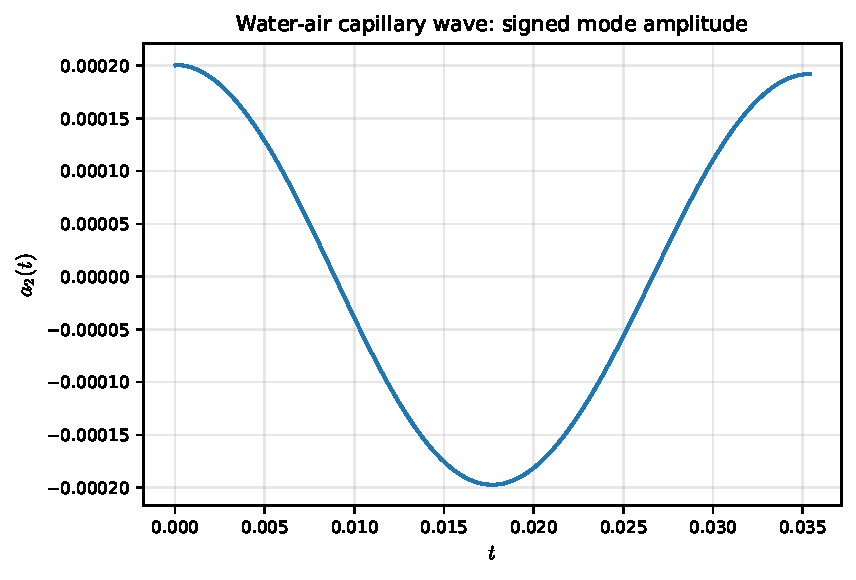
\includegraphics[width=0.32\linewidth]{figures/ch14_capillary_signed_interface_amplitude.pdf}
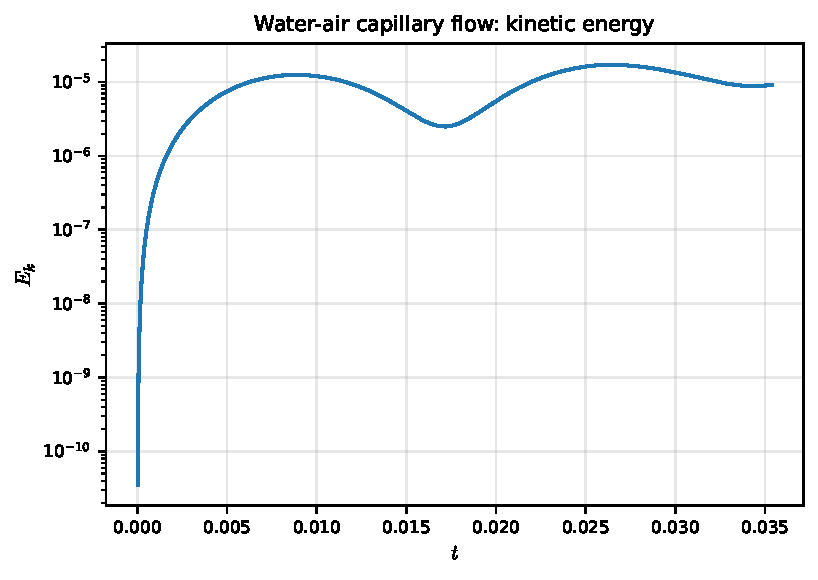
\includegraphics[width=0.32\linewidth]{figures/ch14_capillary_kinetic_energy.pdf}
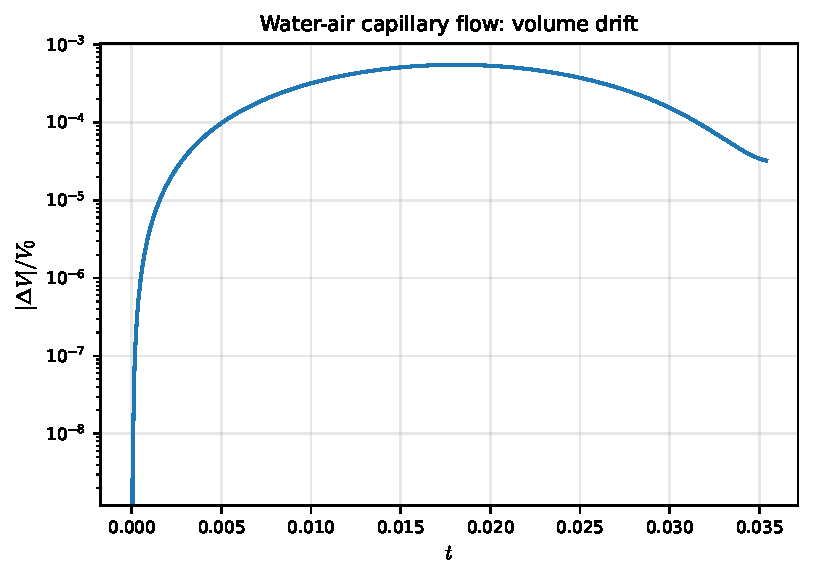
\includegraphics[width=0.32\linewidth]{figures/ch14_capillary_volume_drift.pdf}
\caption{N=32，毛管波掲載窓の時系列診断．左から，符号付き mode-2 界面振幅，
運動エネルギー，体積ドリフトを示す．}
\label{fig:ch14_capillary_histories}
\end{figure}

2 次元場としては，\autoref{fig:ch14_capillary_psi_snapshots} に
界面形状の掲載窓推移を示し，
\autoref{fig:ch14_capillary_velocity_pressure_snapshots} に速度場と
圧力 Hodge 代表を示す．
速度 snapshot の最大速度は $7.588\times10^{-2}\,\mathrm{m/s}$ であり，
終端では同じ上側最大位相に戻りつつ，粘性散逸と粗格子表現により
初期振幅よりわずかに小さい．
さらに終端 snapshot では壁面法線速度と $x$ 周期端の速度 mismatch は
いずれも $0$ であった．
圧力 snapshot は界面近傍の Hodge 代表として読み，
diffuse interface を滑らかに塗りつぶした絶対圧分布としては解釈しない．

\begin{figure}[!htbp]
\centering
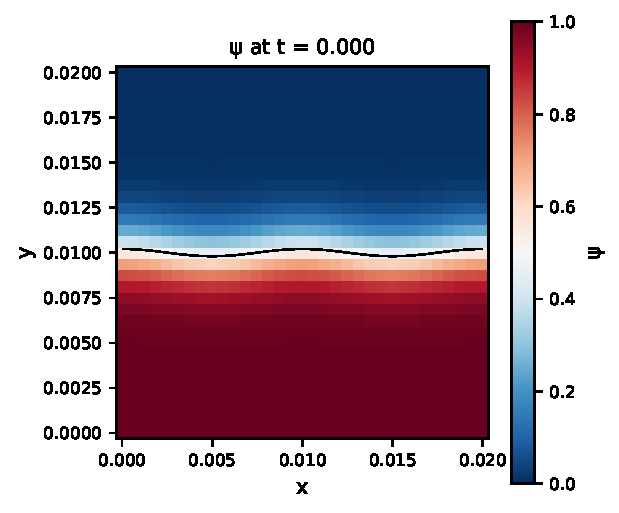
\includegraphics[width=0.19\linewidth]{figures/ch14_capillary_psi_t0.pdf}
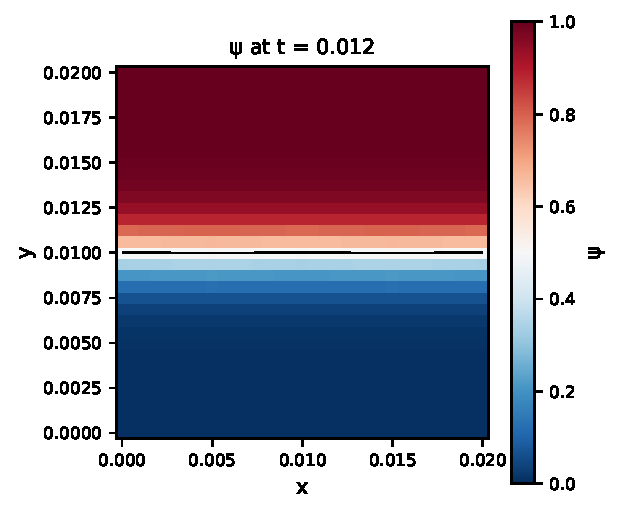
\includegraphics[width=0.19\linewidth]{figures/ch14_capillary_psi_tq1.pdf}
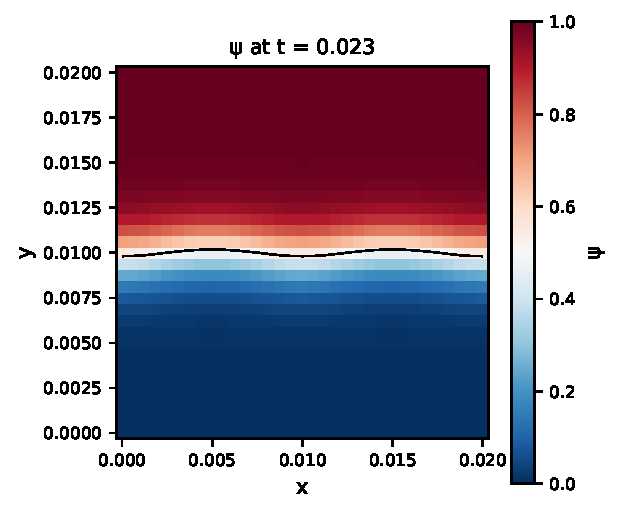
\includegraphics[width=0.19\linewidth]{figures/ch14_capillary_psi_tq2.pdf}
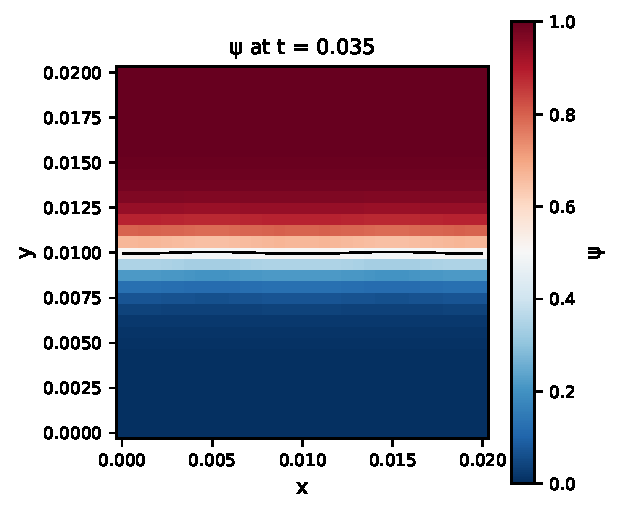
\includegraphics[width=0.19\linewidth]{figures/ch14_capillary_psi_tq3.pdf}
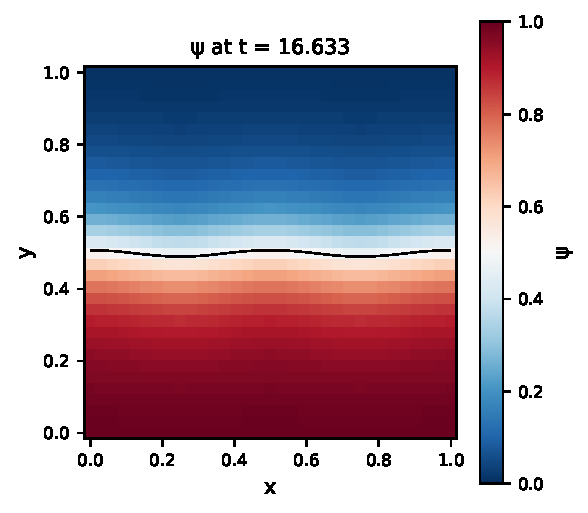
\includegraphics[width=0.19\linewidth]{figures/ch14_capillary_psi_t1.pdf}
\caption{N=32，毛管波の \texorpdfstring{$\psi$}{psi} snapshot．左から
起点，上側最大からのゼロ交差，下側最大，ふたたびゼロ交差，
上側最大へ戻る終点を示す．色軸は全時刻で共通である．}
\label{fig:ch14_capillary_psi_snapshots}
\end{figure}

\begin{figure}[!htbp]
\centering
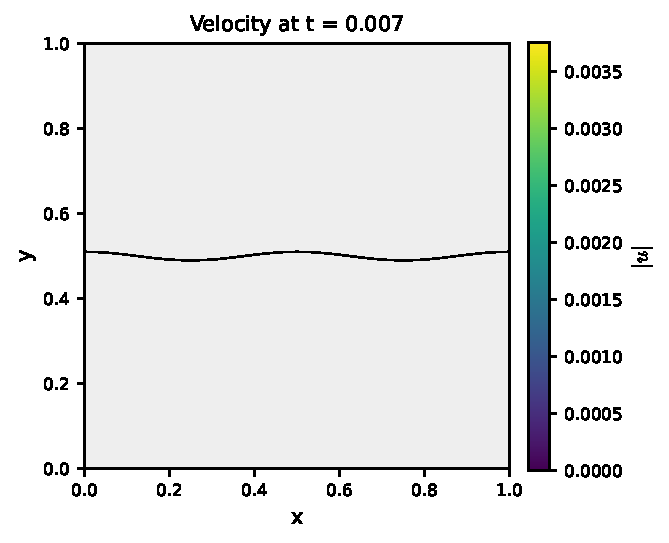
\includegraphics[width=0.19\linewidth]{figures/ch14_capillary_velocity_t0.pdf}
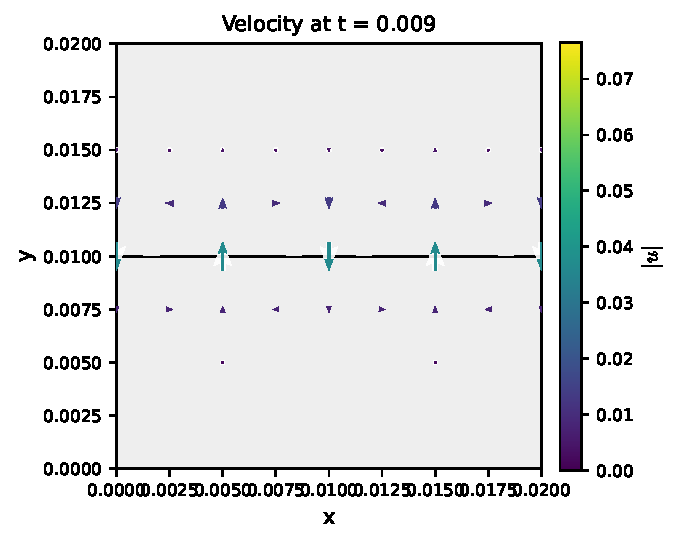
\includegraphics[width=0.19\linewidth]{figures/ch14_capillary_velocity_tq1.pdf}
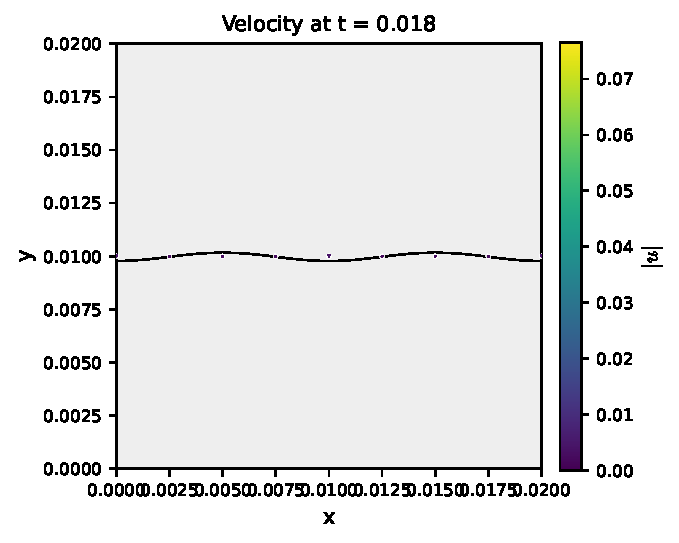
\includegraphics[width=0.19\linewidth]{figures/ch14_capillary_velocity_tq2.pdf}
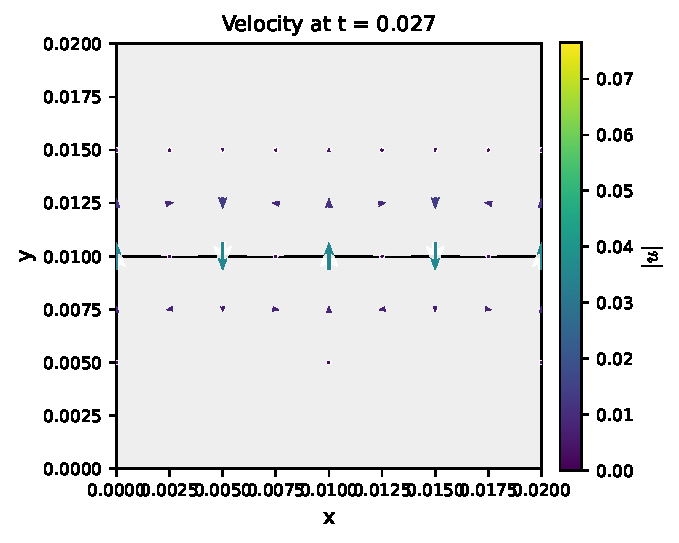
\includegraphics[width=0.19\linewidth]{figures/ch14_capillary_velocity_tq3.pdf}
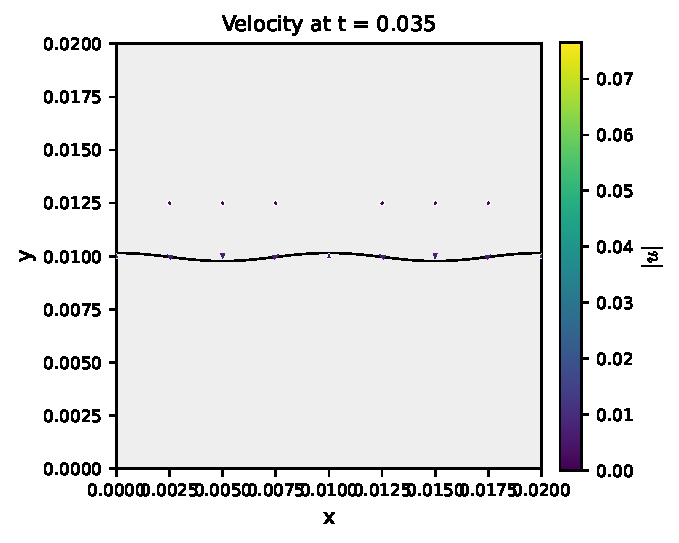
\includegraphics[width=0.19\linewidth]{figures/ch14_capillary_velocity_t1.pdf}
\par\smallskip
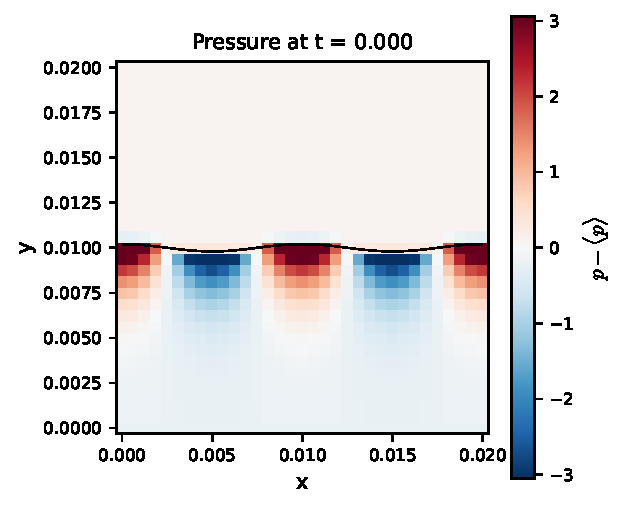
\includegraphics[width=0.19\linewidth]{figures/ch14_capillary_pressure_t0.pdf}
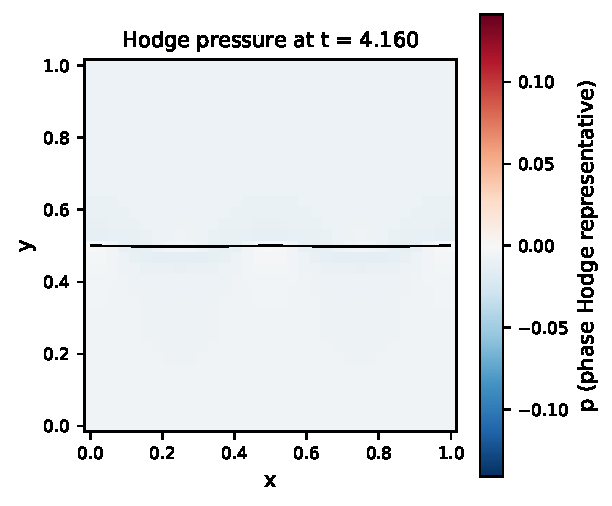
\includegraphics[width=0.19\linewidth]{figures/ch14_capillary_pressure_tq1.pdf}
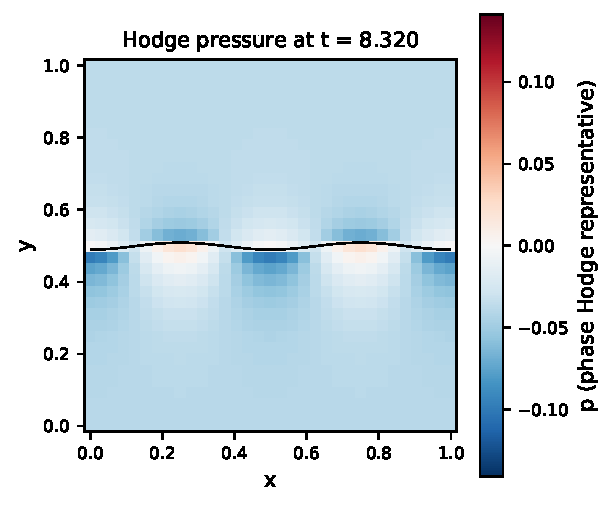
\includegraphics[width=0.19\linewidth]{figures/ch14_capillary_pressure_tq2.pdf}
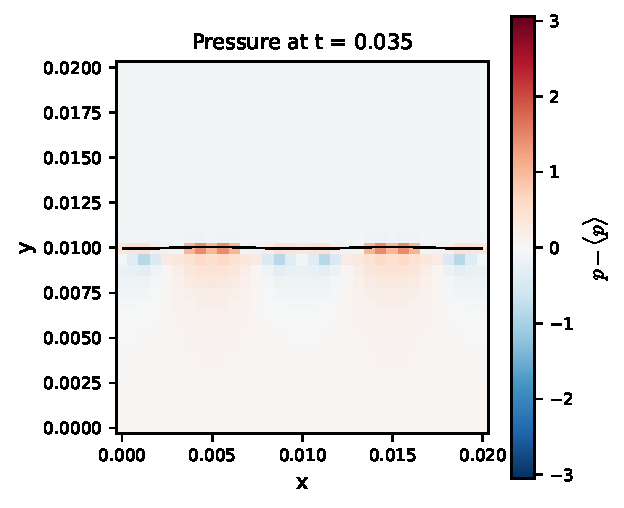
\includegraphics[width=0.19\linewidth]{figures/ch14_capillary_pressure_tq3.pdf}
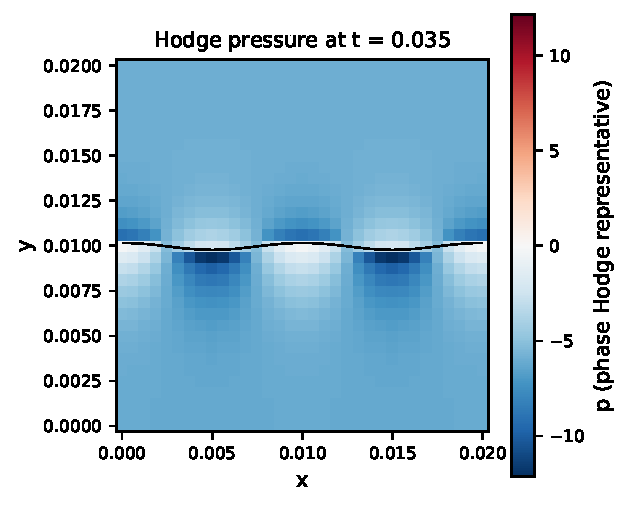
\includegraphics[width=0.19\linewidth]{figures/ch14_capillary_pressure_t1.pdf}
\caption{N=32，毛管波の 2 次元速度場と圧力 Hodge 代表．
上段は速度場，下段は圧力代表であり，左から
起点，上側最大からのゼロ交差，下側最大，ふたたびゼロ交差，
上側最大へ戻る終点を示す．
上段は背景スカラー場を描かず，矢印の長さと色で速度ベクトルを表す．
速度矢印の色軸と矢印スケール，
および圧力色軸はそれぞれ全時刻で共通である．}
\label{fig:ch14_capillary_velocity_pressure_snapshots}
\end{figure}

このケースの判定は，
「平坦界面の毛管剛性が正しい向きで PPE/corrector に伝わり，
幾何セル分率輸送，投影済み面共鎖移送，pressure-coordinate history，
FCCD PPE，IMEX--BDF2 運動量更新が有界な復元振動を保つ」
である．
この結果により，後続の液滴・気泡・Rayleigh--Taylor で用いる
同じ bundle Young--Laplace work と $j_{gl}$ contract を，
界面曲率の符号に対して分岐させずに使える．
ただし，U12 で棄却した全圧力像過射影はこの結果の一部ではない．

% ═══════════════════════════════════════════════════════════════════
\subsection{振動液滴：移流・粘性項を含む閉じた毛管振動}
\label{sec:val_oscillating_droplet}
% ═══════════════════════════════════════════════════════════════════

\subsubsection{設定と理論基準}

振動液滴ベンチマークは，静止 Laplace 圧バランスの再確認ではない．
円形液滴をわずかに楕円へ変形しておき，表面張力が形状を復元する過程で，
界面輸送，運動量対流，粘性散逸，pressure-jump 仕事が同時に働くかを見る．
静止円形液滴は production-stack static gate を含めて第~\ref{sec:verification}章で扱ったため，
ここでは有限速度で動く閉じた界面だけを対象にする．

初期界面は中心 $(0.01,0.01)\,\mathrm{m}$，半軸
$a=5.5\,\mathrm{mm},\ b=4.5\,\mathrm{mm}$ の液相楕円である．
面積等価半径と初期変形量を
\begin{equation}
  R_{\mathrm{eq}}=\sqrt{ab}=4.974937\,\mathrm{mm},
  \qquad
  D_0=\frac{a-b}{a+b}=0.10
  \label{eq:oscillating_droplet_initial}
\end{equation}
と定義する．
2D の $n=2$ Rayleigh--Lamb 基準では
\begin{equation}
  \omega_0^2
  = \frac{n(n^2-1)\sigma}{(\rho_l+\rho_g)R_{\mathrm{eq}}^3},
  \qquad n=2,
  \label{eq:oscillating_droplet_lamb}
\end{equation}
を第一基準とする~\cite{Prosperetti1981}．
物性値は水--空気の実スケール値
$\rho_l=998.2\,\mathrm{kg/m^3}$，
$\rho_g=1.204\,\mathrm{kg/m^3}$，
$\sigma=0.0728\,\mathrm{N/m}$ を用いる．
このとき $\omega_0=59.578473371\,\mathrm{s^{-1}}$ であり，
最終時刻は
\[
  T_\mathrm{RL}=\frac{2\pi}{\omega_0}=0.105460663082\,\mathrm{s}
\]
とし，1 周期分の応答を読む．

\begin{itemize}[noitemsep,leftmargin=2em]
  \item グリッド：$[0,0.02]^2\,\mathrm{m}^2$，$32^2$，
        periodic，interface-fitted $\alpha=2$
  \item 物性：$\rho_l=998.2\,\mathrm{kg/m^3}$，
        $\rho_g=1.204\,\mathrm{kg/m^3}$，
        $\mu_l=1.002\times10^{-3}\,\mathrm{Pa\,s}$，
        $\mu_g=1.825\times10^{-5}\,\mathrm{Pa\,s}$，
        $\sigma=0.0728\,\mathrm{N/m}$，$g=0$
  \item 時間：$T=0.105460663082\,\mathrm{s}$，理論 CFL multiplier $1.0$
  \item 再初期化：Ridge--Eikonal profile restoration を毎 step 適用し，
        動的閉界面では P1 sharp-phase 面積を
        \texttt{sharp\_phase\_volume} constraint の目標量とする
  \item 時系列診断：符号付き変形量，変形量，体積ドリフト，運動エネルギー
  \item snapshot：
        $0,\frac14T_\mathrm{RL},\frac12T_\mathrm{RL},
        \frac34T_\mathrm{RL},T_\mathrm{RL}$ 近傍の $\psi$/速度/圧力場
\end{itemize}

\subsubsection{結果と判定}

N=32 の 1 周期計算は完走し，$3452$ samples で
$t=0.105460663082\,\mathrm{s}$ に到達し，
すべての snapshot field は有限値を保った．
CFL は全区間で毛管制限が支配し，$dt$ は
$2.65\times10^{-5}$--$3.14\times10^{-5}\,\mathrm{s}$ の範囲に留まった．
\texttt{signed\_deformation} は初期離散値
$7.5535\times10^{-2}$ から負側最小値
$-3.4572\times10^{-2}$ へ進み，
1 周期終端で $2.1808\times10^{-2}$ となった．
しかし Rayleigh--Lamb 基準
$D_0\cos(\omega_0T_\mathrm{RL})=1.0\times10^{-1}$ には戻らず，
この run は閉界面振動の受入結果ではない．
これは単なる位相・粘性減衰の問題ではなく，
下の体積診断が示すように閉じた液相領域そのものが長時間で増加しているためである．

\begin{figure}[!htbp]
\centering
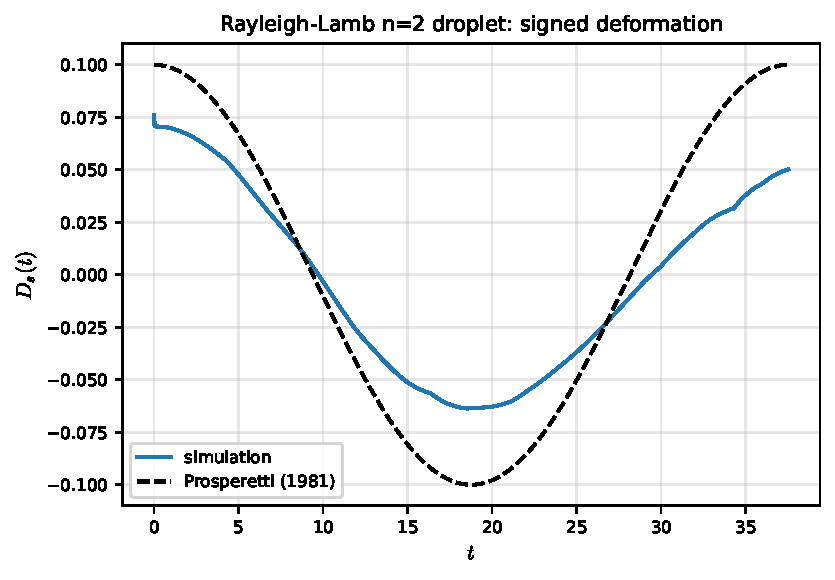
\includegraphics[width=0.32\linewidth]{figures/ch14_osc_droplet_signed_deformation.pdf}
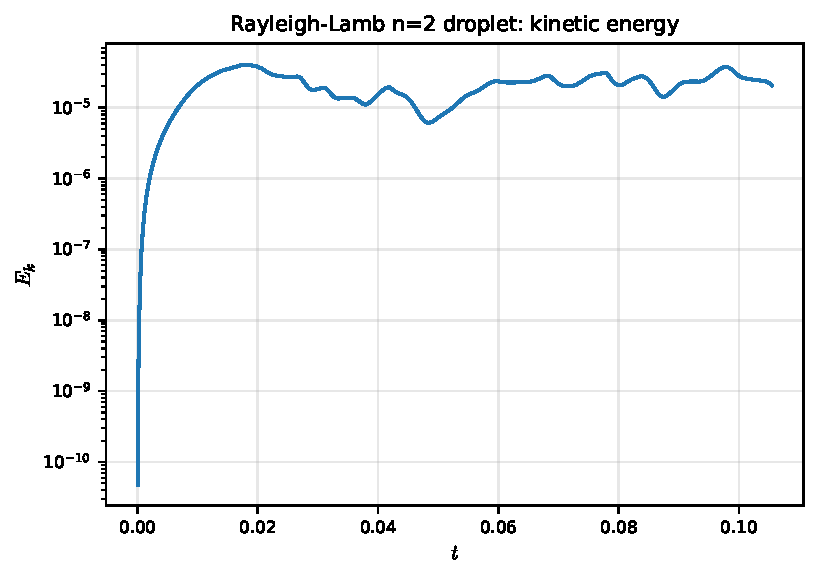
\includegraphics[width=0.32\linewidth]{figures/ch14_osc_droplet_kinetic_energy.pdf}
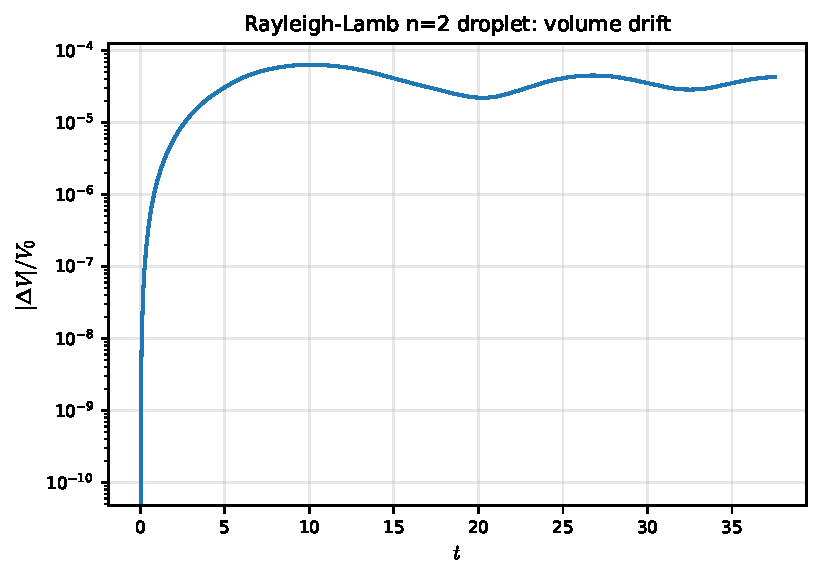
\includegraphics[width=0.32\linewidth]{figures/ch14_osc_droplet_volume_drift.pdf}
\caption{N=32，1 周期振動液滴の時系列診断．左から，符号付き変形量，
運動エネルギー，体積ドリフトを示す．}
\label{fig:ch14_osc_droplet_histories}
\end{figure}

保存量 gate は不合格である．
既存の \texttt{volume\_conservation} 診断は終端で
$3.5495\times10^{-1}$ に達した．
さらに saved snapshot と各時刻の非一様格子座標から P1 marching-squares
sharp area を再構成すると，
最初の snapshot の
$7.7395\times10^{-5}\,\mathrm{m^2}$ から終端
$9.7435\times10^{-5}\,\mathrm{m^2}$ へ増え，
相対ドリフトは $+25.8919\%$ であった．
\texttt{sharp\_phase\_volume} 制約を短時間 probe で満たしていても，
1 周期では transport，dynamic grid rebuild/remap，profile retraction の
合成写像が閉界面体積を保存していない．
\texttt{kinetic\_energy} は
$4.76\times10^{-11}$ から立ち上がって最大
$4.2813\times10^{-5}$，終端
$3.2758\times10^{-5}$ の有界な交換として現れた．
ただし，この有界性は体積保存 gate の失敗を相殺しない．
snapshot の速度最大値は $1.06\times10^{-1}\,\mathrm{m/s}$ であり，
保存された圧力代表も有限範囲に収まった．
したがって，この run の判定は
「有限値で完走したが，閉界面保存量の受入基準を満たさない」である．
2 次元場としては，\autoref{fig:ch14_osc_droplet_psi_snapshots} に界面形状の
1 周期推移を示し，
\autoref{fig:ch14_osc_droplet_velocity_pressure_snapshots} に速度場と
保存された圧力代表を示す．

\begin{figure}[!htbp]
\centering
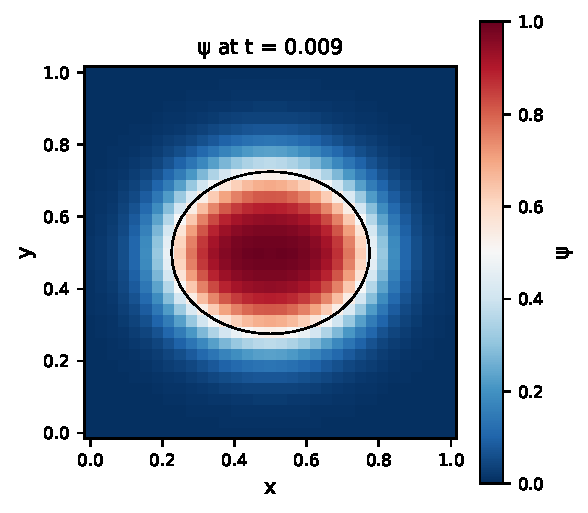
\includegraphics[width=0.19\linewidth]{figures/ch14_osc_droplet_psi_t0.pdf}
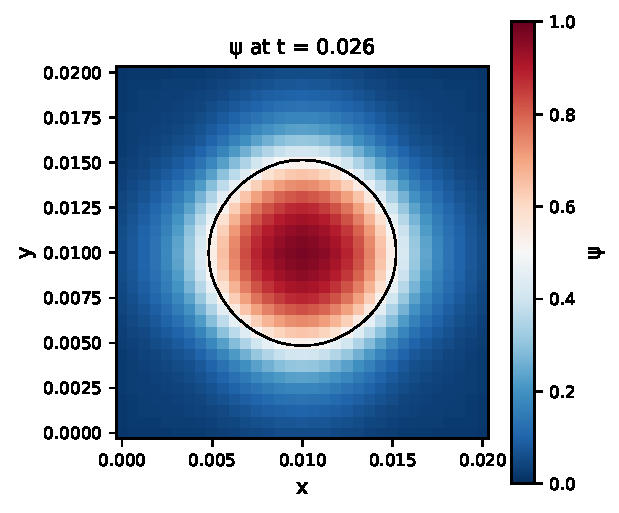
\includegraphics[width=0.19\linewidth]{figures/ch14_osc_droplet_psi_tq1.pdf}
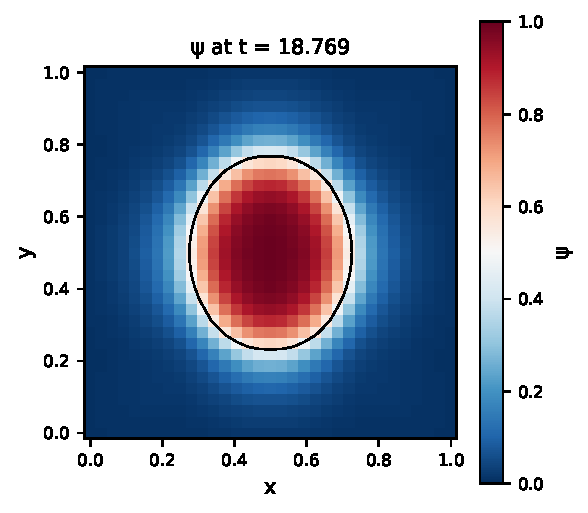
\includegraphics[width=0.19\linewidth]{figures/ch14_osc_droplet_psi_tq2.pdf}
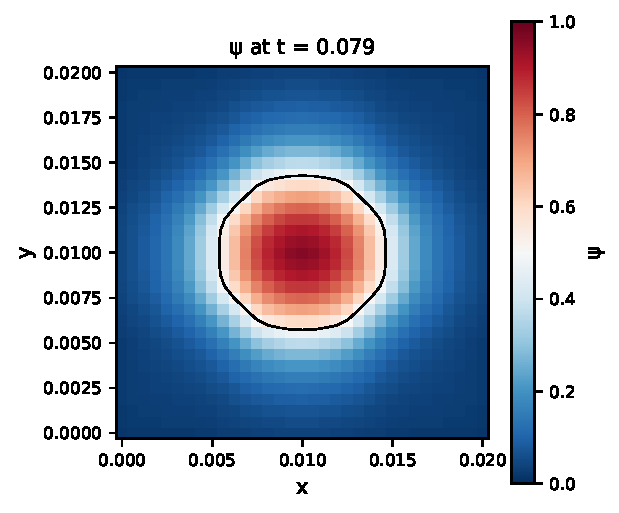
\includegraphics[width=0.19\linewidth]{figures/ch14_osc_droplet_psi_tq3.pdf}
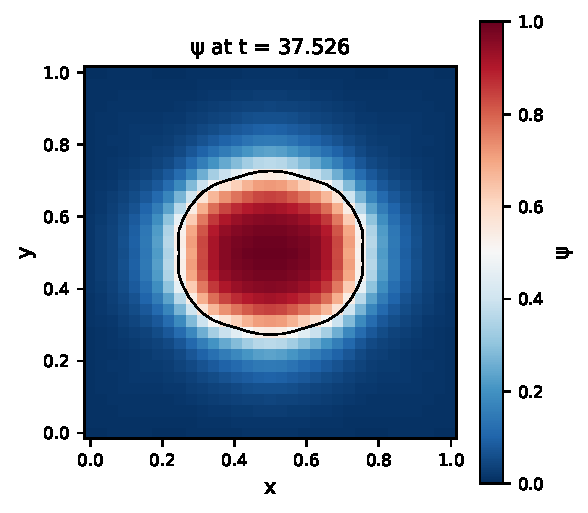
\includegraphics[width=0.19\linewidth]{figures/ch14_osc_droplet_psi_t1.pdf}
\caption{N=32，1 周期振動液滴の \texorpdfstring{$\psi$}{psi} snapshot．左から
\texorpdfstring{$t\approx0,\frac14T_\mathrm{RL},\frac12T_\mathrm{RL},
\frac34T_\mathrm{RL},T_\mathrm{RL}$}{t approximately 0, 1/4 T_RL, 1/2 T_RL, 3/4 T_RL, T_RL} を示す．色軸は全時刻で共通である．}
\label{fig:ch14_osc_droplet_psi_snapshots}
\end{figure}

\begin{figure}[!htbp]
\centering
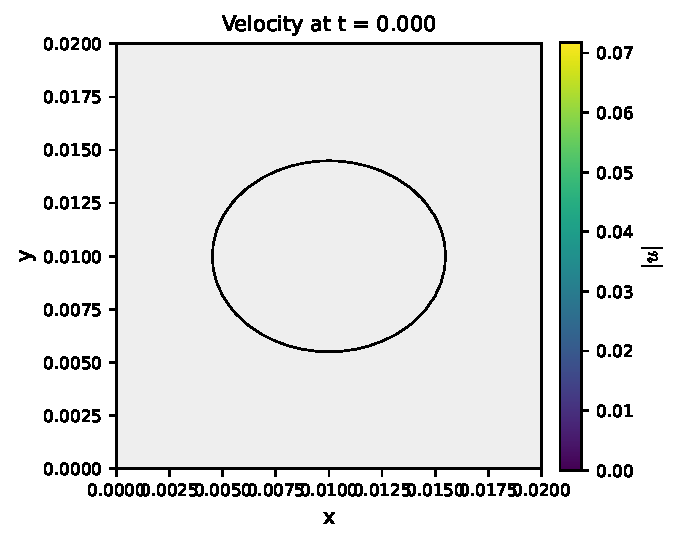
\includegraphics[width=0.19\linewidth]{figures/ch14_osc_droplet_velocity_t0.pdf}
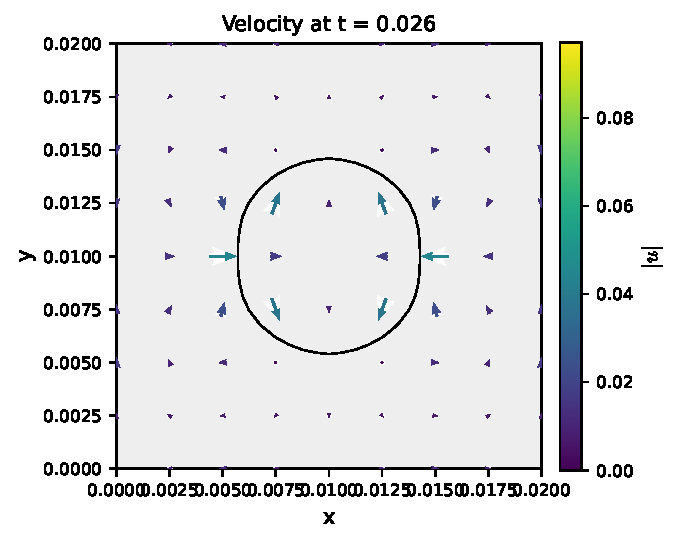
\includegraphics[width=0.19\linewidth]{figures/ch14_osc_droplet_velocity_tq1.pdf}
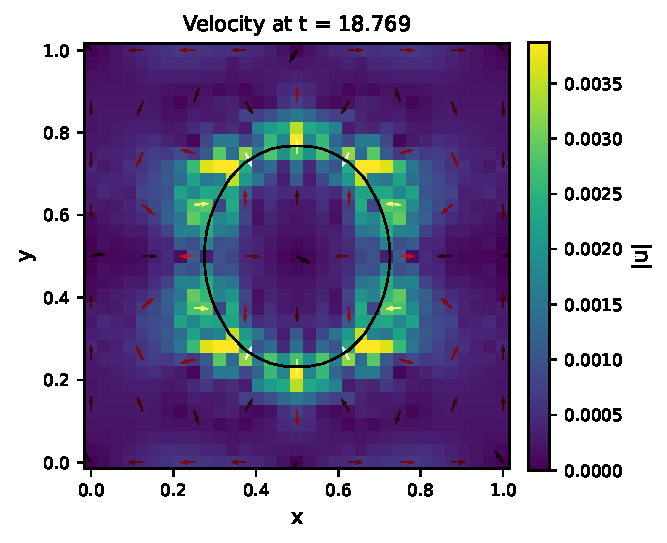
\includegraphics[width=0.19\linewidth]{figures/ch14_osc_droplet_velocity_tq2.pdf}
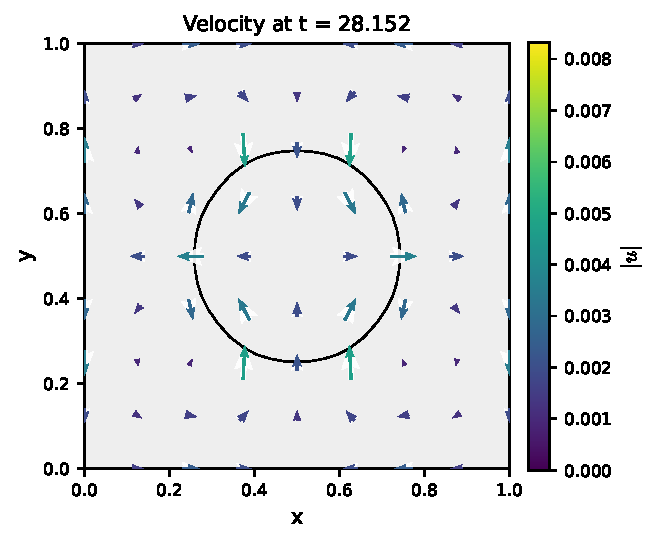
\includegraphics[width=0.19\linewidth]{figures/ch14_osc_droplet_velocity_tq3.pdf}
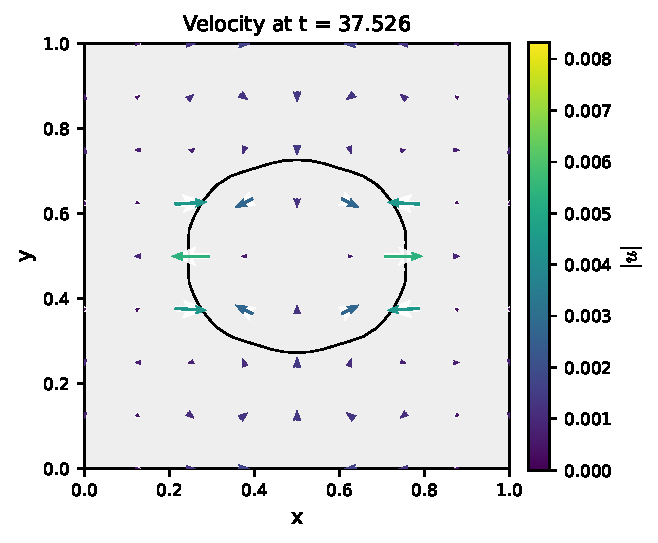
\includegraphics[width=0.19\linewidth]{figures/ch14_osc_droplet_velocity_t1.pdf}
\par\smallskip
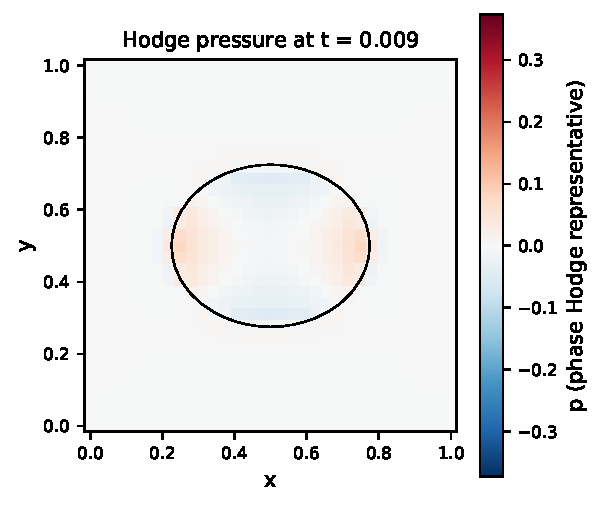
\includegraphics[width=0.19\linewidth]{figures/ch14_osc_droplet_pressure_t0.pdf}
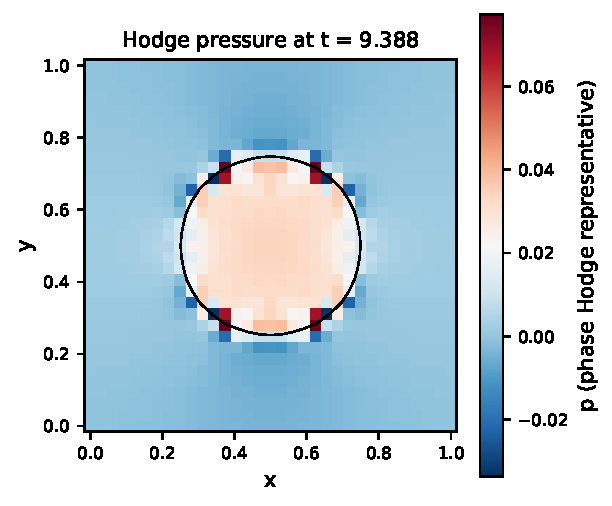
\includegraphics[width=0.19\linewidth]{figures/ch14_osc_droplet_pressure_tq1.pdf}
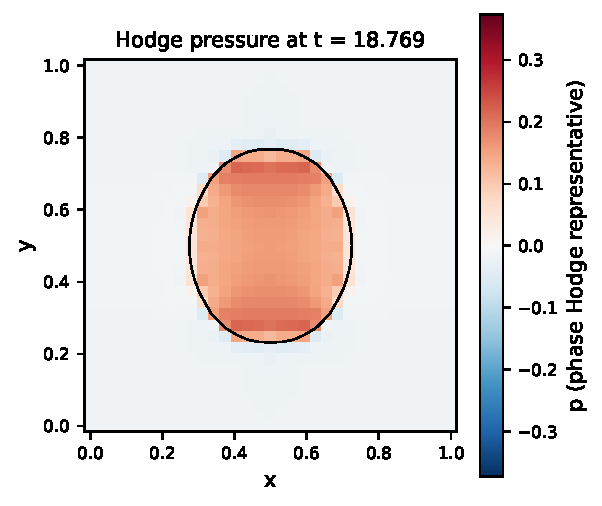
\includegraphics[width=0.19\linewidth]{figures/ch14_osc_droplet_pressure_tq2.pdf}
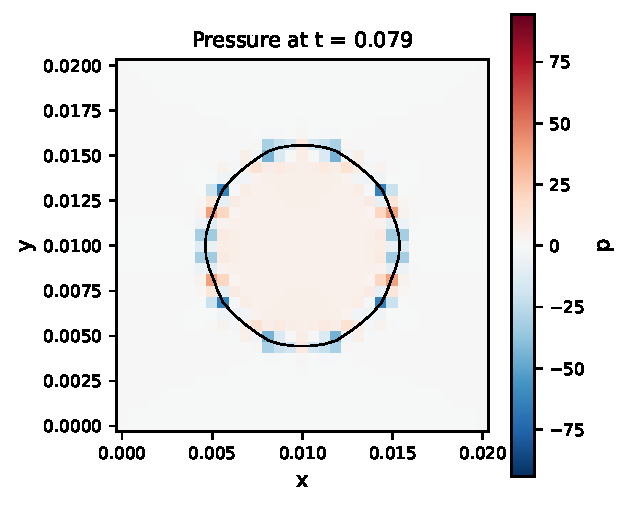
\includegraphics[width=0.19\linewidth]{figures/ch14_osc_droplet_pressure_tq3.pdf}
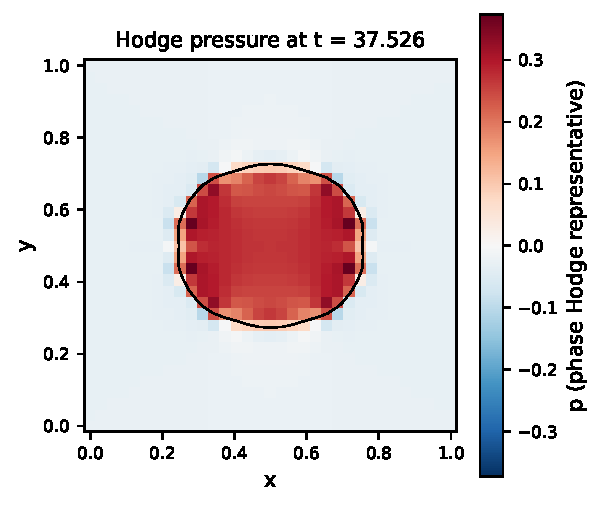
\includegraphics[width=0.19\linewidth]{figures/ch14_osc_droplet_pressure_t1.pdf}
\caption{N=32，1 周期振動液滴の 2 次元速度場と保存された圧力代表．
上段は速度場，下段は圧力代表であり，左から
$t\approx0,\frac14T_\mathrm{RL},\frac12T_\mathrm{RL},
\frac34T_\mathrm{RL},T_\mathrm{RL}$ を示す．
上段は背景スカラー場を描かず，矢印の長さと色で速度ベクトルを表す．
速度矢印の色軸と矢印スケール，
および圧力色軸はそれぞれ全時刻で共通である．}
\label{fig:ch14_osc_droplet_velocity_pressure_snapshots}
\end{figure}

本ケースから得る結論は成功主張ではなく，未達として残る課題である．
毛管波が平坦界面の符号検証なら，振動液滴は移流・粘性項を含む
閉界面エネルギー交換と保存量整合のベンチマークである．
現状の標準構成は，1 周期の楕円液滴に対して
bounded run を作る一方で，sharp 体積を保存する離散写像としては閉じていない．
したがって次の修正対象は，P1 area を状態変数として持つ
transport/remap/retraction の同一 cochain 化であり，
拡散質量や見た目の楕円振幅で代用してはならない．

% ═══════════════════════════════════════════════════════════════════
\subsection{単一気泡上昇：浮力残差と projection の共有}
\label{sec:val_rising_bubble}
% ═══════════════════════════════════════════════════════════════════

\subsubsection{設定と理論的焦点}

単一気泡上昇ベンチマークでは，水中に空気円を置き，
実重力下で上昇させる．
幾何は Hysing 型の単一気泡配置~\cite{Hysing2009}を参照するが，
物性と長さは $10\,\mathrm{mm}$ 級の水--空気系へ戻し，
目的を「終端速度表の再現」だけに置かない．
本ケースの焦点は，表面張力の pressure-jump 閉包と，
浮力分解
\[
  \rho\bm{g}=-\bnabla(\rho\Phi_g)+\Phi_g\bnabla\rho
\]
から得る face residual acceleration が，同じ projection 空間で閉じるかにある．
hydrostatic な勾配成分を nodal predictor に直接入れると，
projection で消えるべき力が非ソレノイダル速度として残る．
したがって浮力残差は，PPE と同じ $A_f,G_f,D_f$ 上で評価する．

\begin{itemize}[noitemsep,leftmargin=2em]
  \item グリッド：$[0,0.01]\times[0,0.02]\,\mathrm{m}$，
        $32\times64$，$x$ 周期/$y$ 壁面，static interface-fitted $\alpha=2$
  \item 初期界面：中心 $(0.005,0.005)\,\mathrm{m}$，
        半径 $R=0.0025\,\mathrm{m}$ の気泡
  \item 物性：$\rho_l=1000$，$\rho_g=1.2$，
        $\mu_l=10^{-3}$，$\mu_g=1.8\times10^{-5}$，
        $\sigma=0.072$，$g=9.81$
  \item 時間：掲載窓 $0\le t\le0.03\,\mathrm{s}$，
        snapshot は $0.005\,\mathrm{s}$ 刻み，理論 CFL multiplier $1.0$
  \item 出力：\texttt{bubble\_centroid}，
        \texttt{mean\_rise\_velocity}，\texttt{deformation}，
        \texttt{volume\_conservation}，$\psi$/速度/圧力 snapshot
\end{itemize}

\subsubsection{結果と判定}

図~\ref{fig:ch14_rising_bubble_initial_snapshots}に，
現在の論文に掲載する初期窓の $\psi$ snapshot を示す．
$t=0.0299956\,\mathrm{s}$ では，重心は
$y_c=7.350\times10^{-3}\,\mathrm{m}$，
平均上昇速度は $9.57\times10^{-2}\,\mathrm{m/s}$，
変形量は $D=0.343$ であり，
diffuse phase-volume drift は $8.99\times10^{-6}$ に留まる．
したがって $0\le t\le0.03\,\mathrm{s}$ の範囲では，
相体積の漏れではなく，浮力残差と粘性抵抗・表面張力閉包の釣合いとして
初期上昇と変形を読むことができる．

\begin{figure}[!htbp]
\centering
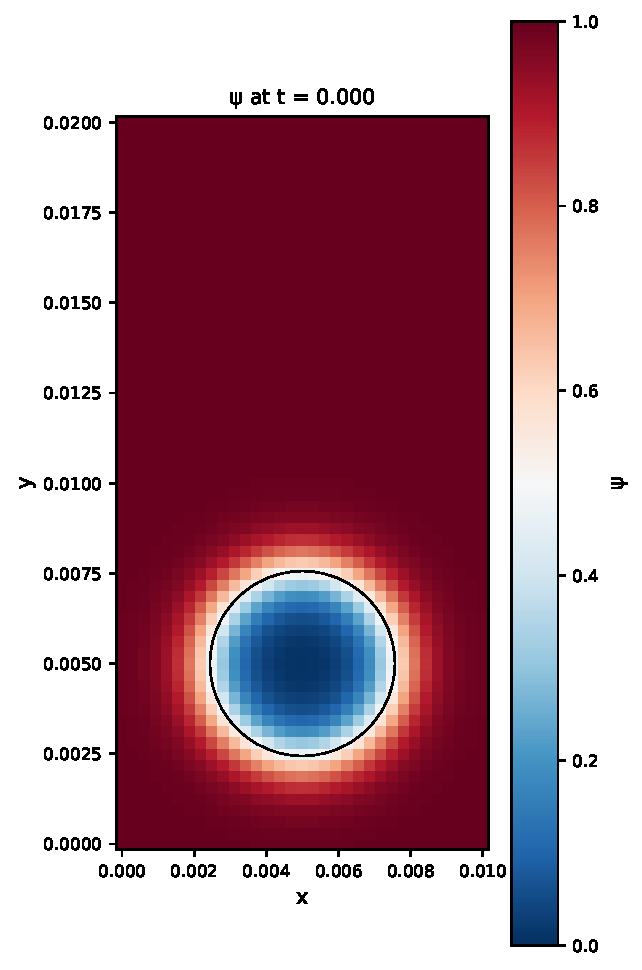
\includegraphics[width=0.23\linewidth]{figures/ch14_rising_bubble_psi_t000.pdf}
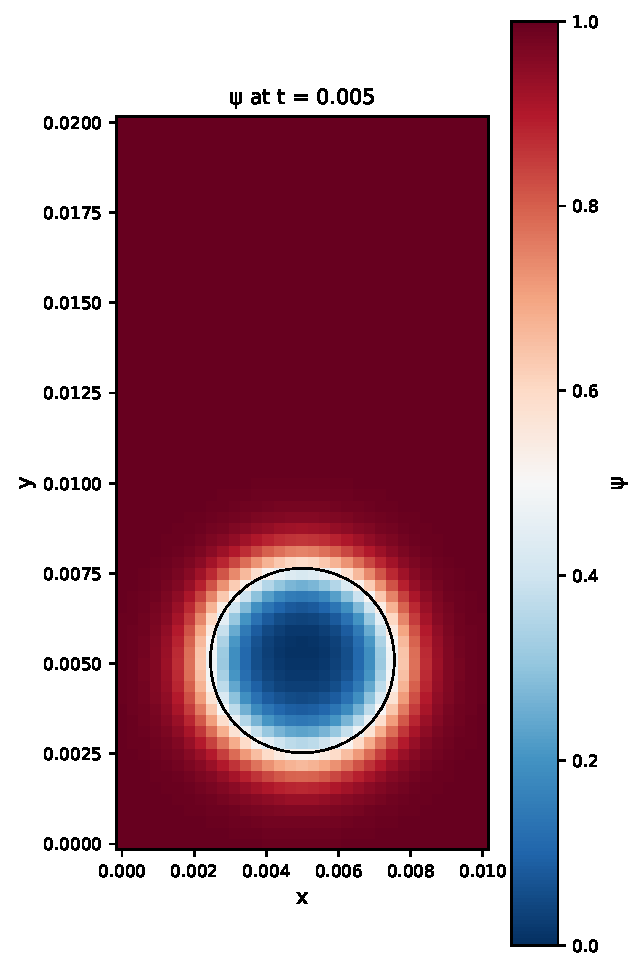
\includegraphics[width=0.23\linewidth]{figures/ch14_rising_bubble_psi_t005.pdf}
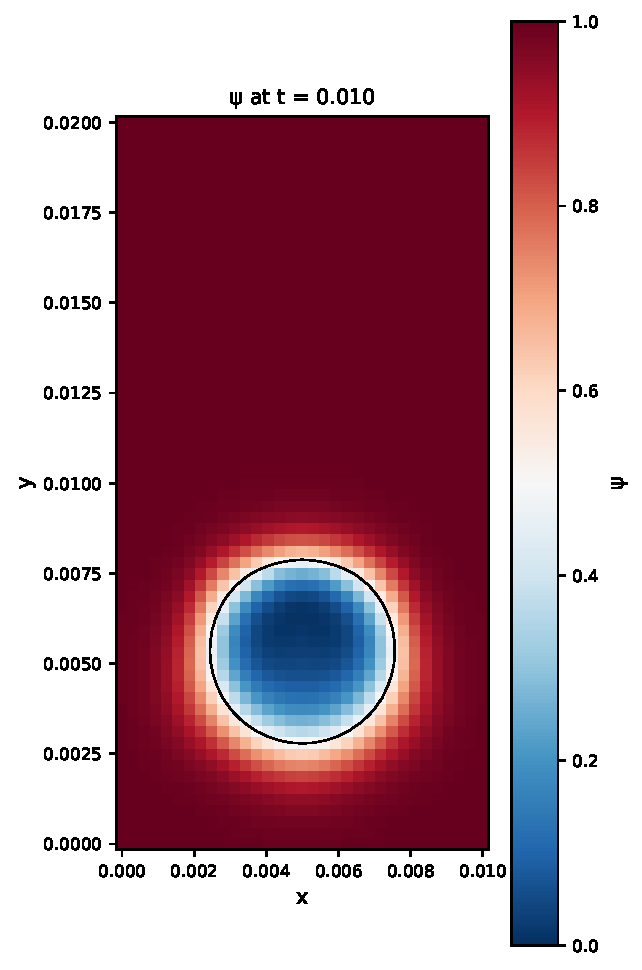
\includegraphics[width=0.23\linewidth]{figures/ch14_rising_bubble_psi_t010.pdf}
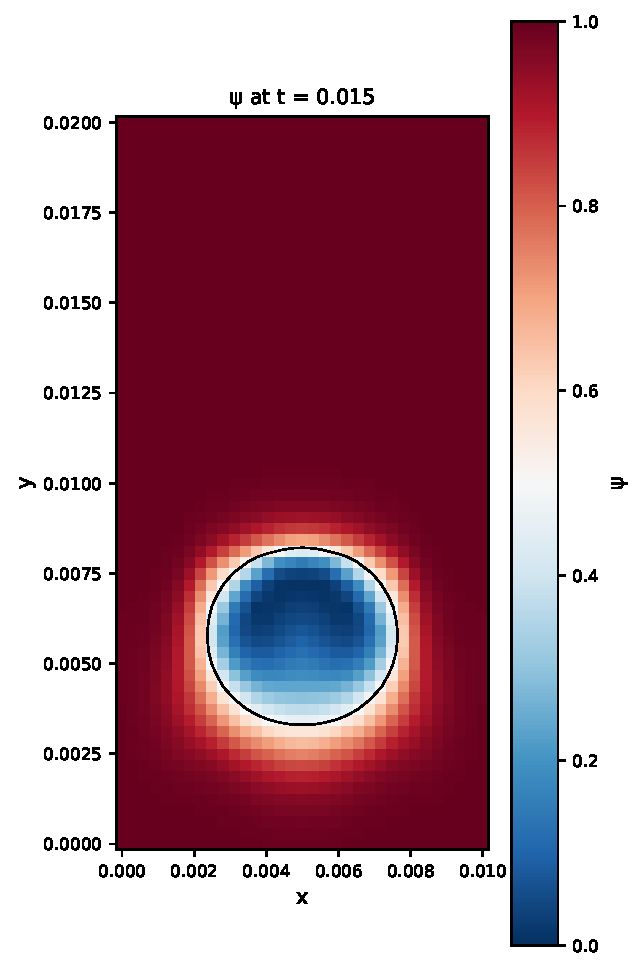
\includegraphics[width=0.23\linewidth]{figures/ch14_rising_bubble_psi_t015.pdf}\\[-0.2em]
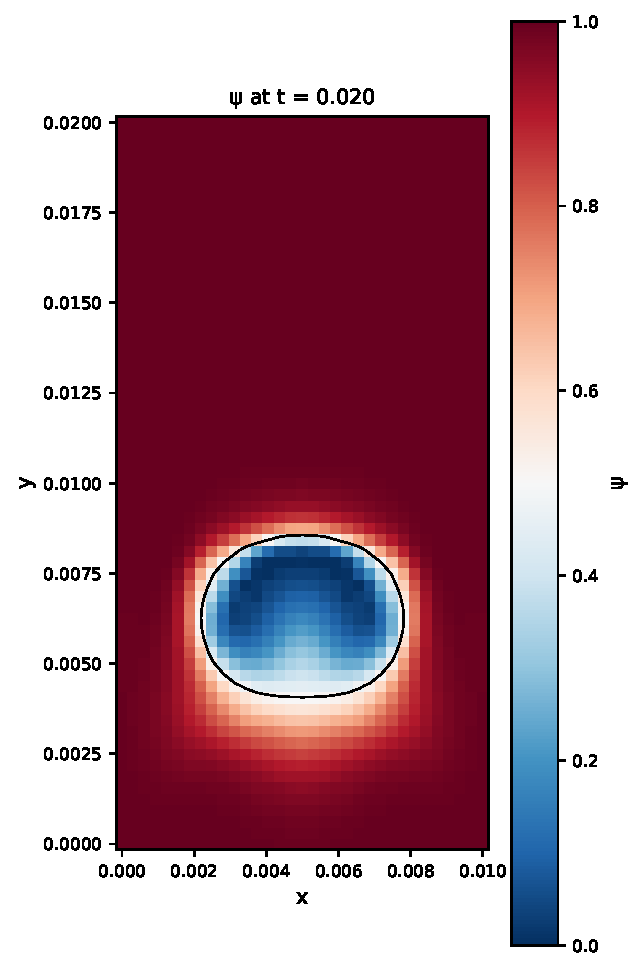
\includegraphics[width=0.23\linewidth]{figures/ch14_rising_bubble_psi_t020.pdf}
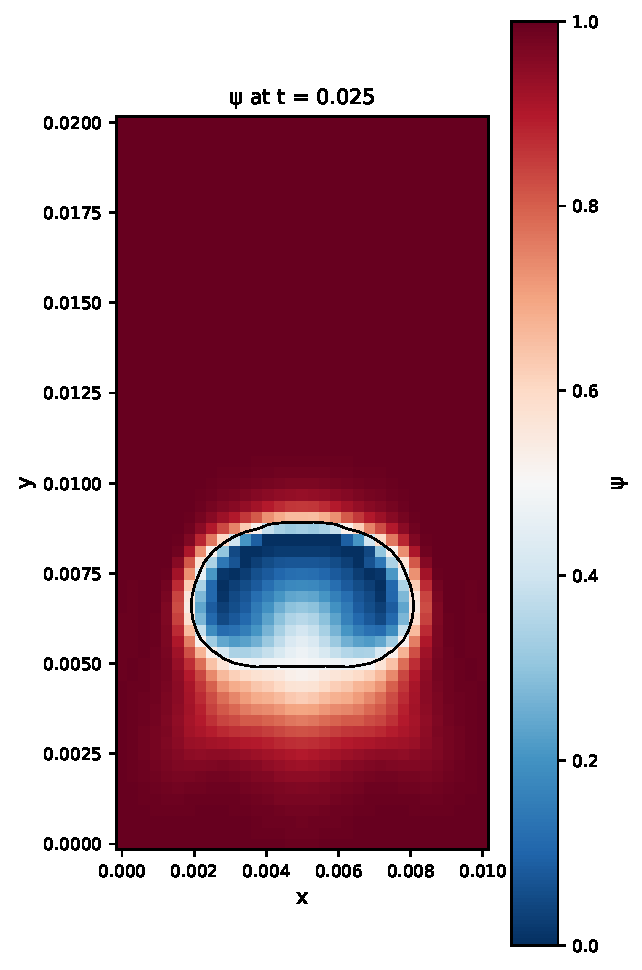
\includegraphics[width=0.23\linewidth]{figures/ch14_rising_bubble_psi_t025.pdf}
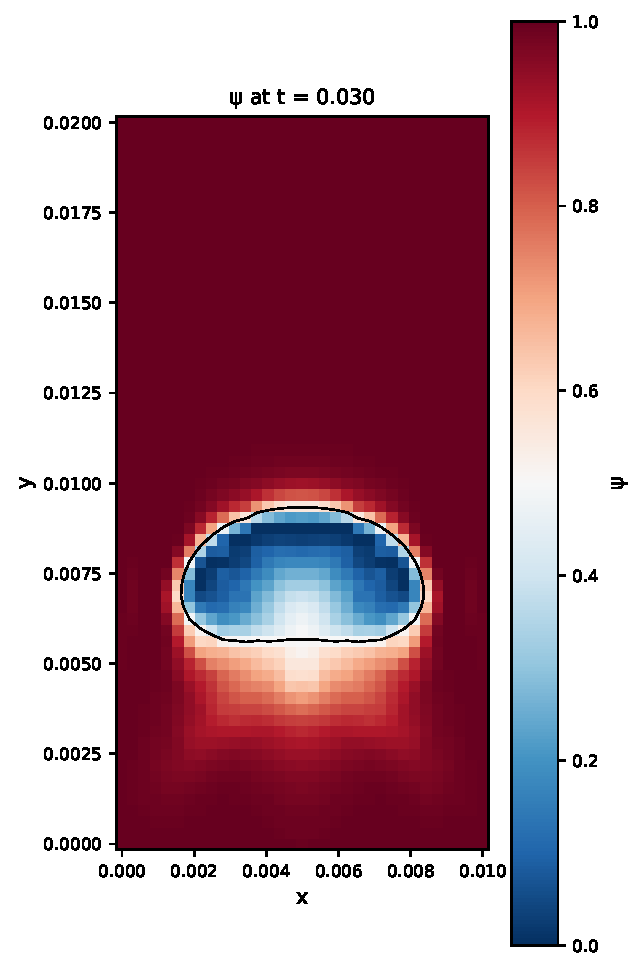
\includegraphics[width=0.23\linewidth]{figures/ch14_rising_bubble_psi_t030.pdf}
\caption{単一気泡上昇の掲載 snapshot．
左上から $t=0,0.005,\ldots,0.03\,\mathrm{s}$ の $\psi$ 場を示す．
本稿では形状破綻が顕在化する前の初期窓だけを掲載対象とする．}
\label{fig:ch14_rising_bubble_initial_snapshots}
\end{figure}

一方，継続計算では $t\simeq0.04\,\mathrm{s}$ 以降に
下側界面の停滞と $\psi=0.5$ 形状の分裂が見え始める．
この破れは，diffuse phase-volume diagnostic が小さいままでも
sharp gas geometry と連結性が保存されないという，
保存すべき不変量の取り違えを示している．
したがって長時間の気泡形状・終端速度ベンチマークとしては採用せず，
幾何 cell-fraction state space で
material volume と gauge profile の互換性を同一 cochain に戻す課題として扱う．

本ケースの判定は，
「$0\le t\le0.03\,\mathrm{s}$ の初期窓では
surface-tension pressure-jump と hydrostatic-balanced buoyancy が
同じ面速度空間の射影に入り，上昇応答を作る．
ただし $t\simeq0.04\,\mathrm{s}$ 以降の形状保存は未解決であり，
本章の合格 claim には含めない」
である．

% ═══════════════════════════════════════════════════════════════════
\subsection{Rayleigh--Taylor 不安定性：線形成長から非線形形状へ}
\label{sec:val_rayleigh_taylor}
% ═══════════════════════════════════════════════════════════════════

\subsubsection{設定と理論基準}

Rayleigh--Taylor ベンチマークでは，水（重相，上）／シリコーン油 5cSt（軽相，下）の
二層配置に小振幅摂動を与え，重力下で不安定成長させる．
本稿の記号規約では，
液相記号を下層シリコーン油，
気相記号を上層水に対応させる．
これは物理相の密度順序を優先するための記号規約であり，
pressure-jump の向き $j_{gl}=p_g-p_l$ は他ケースと同じままである．

線形理論では，小振幅擾乱 $A_0$ は
\begin{equation}
  A(t) = A_0 \, e^{\gamma t},
  \qquad
  \gamma = \sqrt{\mathrm{At}\, g\, k},
  \qquad
  \mathrm{At} = \frac{\rho_{\text{w}}-\rho_{\text{oil}}}{\rho_{\text{w}}+\rho_{\text{oil}}},
  \qquad
  k = \frac{2\pi m}{L_x}
  \label{eq:rt_linear_growth}
\end{equation}
を第一基準に置く~\cite{Chandrasekhar1961}．
本設定では
$\mathrm{At}\approx0.0256$，$k=4\pi$，
$\gamma\approx1.78\,\mathrm{s^{-1}}$ であり，
$T=7.0$ は線形領域を越えて非線形 mushroom 形成を観察する時間である．

\begin{itemize}[noitemsep,leftmargin=2em]
  \item グリッド：$[0,0.5]\times[0,2.0]$，$128\times512$，
        壁面境界，interface-fitted $\alpha=2$
  \item 物性：下層シリコーン油 $\rho=950,\mu=5\times10^{-3}$；
        上層水 $\rho=1000,\mu=10^{-3}$
  \item 表面張力・重力：$\sigma=0.040$，$g=9.81$
  \item 初期界面：$y_0=1.0$，$A_0=0.01$，$m=1$，$L_x=0.5$
  \item 時間：$T=7.0$，理論 CFL multiplier $1.0$
  \item 出力：\texttt{interface\_amplitude}，
        \texttt{kinetic\_energy}，\texttt{volume\_conservation}，
        $\psi$/速度/圧力 snapshot
\end{itemize}

\subsubsection{結果と判定}

早期窓では，\texttt{interface\_amplitude} が
式~\eqref{eq:rt_linear_growth} の対数線形増幅と整合する．
その後，snapshot 上では spike/bubble 構造が発達し，
運動エネルギーは線形増幅に伴って増加したのち，非線形領域で有界な推移へ移る．
体積保存が保たれることで，mushroom 形状は相体積の数値漏れではなく，
浮力不安定性の形状発展として読める．

本ケースの判定は，
「pressure-jump と hydrostatic-balanced buoyancy を同じ stack で使ったまま，
安定振動だけでなく不安定成長も正しい向きに発生させられる」
である．
毛管波・振動液滴が表面張力主導の復元問題であるのに対し，
Rayleigh--Taylor は浮力主導の成長問題であり，
同じ面速度空間の契約が両方を支えることを示した．

% ═══════════════════════════════════════════════════════════════════
\subsection{総括}
\label{sec:val_summary}
% ═══════════════════════════════════════════════════════════════════

\begin{table}[htbp]
\centering
\caption{第~\ref{sec:validation}章の物理ベンチマークと判定軸}
\label{tab:ch14_summary}
\PaperTableDenseSetup
\begin{tabular}{>{\raggedright\arraybackslash}p{2.8cm}>{\raggedright\arraybackslash}p{3.6cm}>{\raggedright\arraybackslash}p{5.2cm}>{\raggedright\arraybackslash}p{1.8cm}}
\toprule
ベンチマーク & 条件 & 主に読む診断 & 判定 \\
\midrule
毛管波 &
  $32^2$，$T=0.035379718894\,\mathrm{s}$，水--空気，
  $\lambda=10\,\mathrm{mm}$，$x$ 周期/$y$ 壁面 &
  \texttt{signed\_interface\_amplitude} の復元位相，
  \texttt{kinetic\_energy} の有界振動，
  \texttt{volume\_conservation} &
  \checkmark \\
振動液滴 &
  $32^2$，$T=0.105460663082\,\mathrm{s}$，水--空気，
  periodic，$D_0=0.10$ &
  \texttt{signed\_deformation}，
  \texttt{volume\_conservation}，
  P1 sharp area，運動エネルギー交換 &
  未合格 \\
単一気泡上昇 &
  $32\times64$，掲載窓 $0\le t\le0.03\,\mathrm{s}$，
  $10\,\mathrm{mm}\times20\,\mathrm{mm}$，水--空気，$g=9.81$ &
  $y_c(t)$，\texttt{mean\_rise\_velocity}，
  \texttt{deformation}，diffuse 体積保存，$\psi$ snapshot，
  $t\simeq0.04\,\mathrm{s}$ 以降の形状破綻 &
  初期窓のみ \\
Rayleigh--Taylor &
  $128\times512$，$T=7$，水/シリコーン油，$g=9.81$ &
  \texttt{interface\_amplitude} の線形成長率，
  mushroom 形成，\texttt{kinetic\_energy}，体積保存 &
  \checkmark \\
\bottomrule
\end{tabular}
\end{table}

4 本のベンチマークは，同じ標準構成を
異なる物理機構へ置いたときの成功条件を分担している．
毛管波は pressure-jump の符号と毛管復元力を確認した．
振動液滴は，有限値で 1 周期完走する一方，
P1 sharp area が終端で $+25.9\%$ 増えるため，
閉界面保存量の同一 cochain 化がまだ不足していることを示した．
単一気泡上昇は，$0\le t\le0.03\,\mathrm{s}$ の初期窓で
浮力残差と射影が同じ面速度空間を共有することを確認したが，
後続時刻の形状保存は未解決として合格 claim から外した．
Rayleigh--Taylor は，復元ではなく不安定成長を起こす配置でも
同じ閉包が形状発展を支えることを示した．
したがって本章の結論は，個別部品が単体で正しいだけでなく，
移動界面二相流の代表的な安定振動・初期浮力上昇・不安定成長に対して
同じ stack が有効に働く範囲と，閉界面振動でなお破れている
保存量契約および気泡長時間形状保存の境界を同時に示した，という点にある．
